% =====================================================================
%  Climate Solutions and Strategies | Assignment 1
%  Policy memo: Why limiting climate change matters for Niger
%  Skill Up for Earth, Climate Solutions and Strategies (Fall 2026 cohort)
%  Author: KOUAME Koffi Fidele
%  Compile: lualatex niger_policy_memo.tex (twice)
%  Format: Times New Roman (metric-compatible Liberation Serif), 12 pt, 1.15 line spacing, justified
%  Length: 2 pages including the figure; references on page 3
% =====================================================================
\documentclass[12pt,a4paper]{article}

\usepackage{fontspec}
% Times New Roman if installed, otherwise its metric-compatible equivalent
\IfFontExistsTF{Times New Roman}{\setmainfont{Times New Roman}}{\setmainfont{Liberation Serif}}
\usepackage{setspace}
\setstretch{1.15}
\usepackage[english]{babel}
\usepackage[a4paper,top=2.5cm,bottom=2.5cm,left=2.5cm,right=2.5cm,headsep=0.6cm,footskip=1cm]{geometry}
\usepackage{microtype}
\usepackage{graphicx}
\usepackage{tabularx,array,booktabs}
\usepackage{titlesec}
\usepackage{fancyhdr}
\usepackage{hyperref}
\usepackage{xurl}
\usepackage{caption}
\usepackage{float}
\urlstyle{same}
\hypersetup{colorlinks=true,urlcolor=black,linkcolor=black,citecolor=black,
  pdftitle={Why Limiting Climate Change Matters for Niger},pdfauthor={KOUAME Koffi Fidele}}

% ---- clickable in-text citations (each opens the cited source)
\newcommand{\CIE}{\href{https://climate-impact-explorer.climateanalytics.org}{Climate Analytics, 2026}}
\newcommand{\WBtwentytwo}{\href{http://hdl.handle.net/10986/37620}{World Bank, 2022}}
\newcommand{\WBtwentyfour}{\href{https://www.worldbank.org/en/news/press-release/2024/07/01/the-world-bank-supports-food-security-and-climate-resilience-for-households-in-niger}{World Bank, 2024}}

% ---- layout
\setlength{\parindent}{0pt}
\setlength{\parskip}{5pt}
\captionsetup{font={small,singlespacing},labelfont=bf,skip=3pt,justification=justified,singlelinecheck=false}

\titleformat{\section}{\bfseries}{}{0pt}{}
\titlespacing*{\section}{0pt}{6pt}{1pt}

\pagestyle{fancy}
\fancyhf{}
\fancyhead[L]{\footnotesize\textbf{Climate Solutions and Strategies | Assignment 1}}
\fancyhead[R]{\footnotesize Skill Up for Earth | Fall 2026 | KOUAME Koffi Fidèle}
\fancyfoot[C]{\small\thepage}
\renewcommand{\headrulewidth}{0.6pt}

\newcommand{\degC}{\,\textdegree C}
\newcommand{\rng}[1]{{\footnotesize [#1]}}
\newcolumntype{Y}{>{\raggedright\arraybackslash}X}
\newcolumntype{C}[1]{>{\centering\arraybackslash}p{#1}}

\begin{document}

\begin{center}
{\large\bfseries Policy Memo: Why Limiting Climate Change Matters for Niger}
\end{center}
\vspace{-10pt}

{\small\singlespacing
\renewcommand{\arraystretch}{1.25}
\begin{tabularx}{\linewidth}{|>{\raggedright\arraybackslash}X|>{\raggedright\arraybackslash}X|}
\hline
\textbf{To:} Minister of Environment, Head of Niger's UNFCCC delegation &
\textbf{From:} KOUAME Koffi Fidèle, Climate Adviser \\
\hline
\textbf{Date:} 14 October 2026 &
\textbf{Subject:} Climate risks for Niger and the case for limiting global warming \\
\hline
\end{tabularx}}

\section{Key message}
Models indicate that, under current global policies, Niger could face about 91 days of dangerous heat a year
by 2100, three times today's level, against about 42 if warming is held below 2\degC{} and 32 on a 1.5\degC{}
pathway. Because most Nigeriens farm and herd outdoors, this is the largest loss that faster global emission
cuts can still avoid. Severe drought, by contrast, is projected to become near-universal in every scenario, so
Niger also needs adaptation finance now.

\section{Three priority impacts}
{\small\singlespacing
\renewcommand{\arraystretch}{1.2}
\begin{tabularx}{\linewidth}{@{}Y C{1.75cm} C{2.25cm} C{2.25cm} C{2.25cm}@{}}
\toprule
\textbf{Impact (CIE indicator)} & \textbf{Today (2020)} & \textbf{2100: 1.5\degC{} path} &
\textbf{2100: below 2\degC} & \textbf{2100: current policies}\\
\midrule
Dangerous heat: days per year with a daily maximum heat index above 40\degC &
31\newline\rng{25--38} & 32\newline\rng{24--50} & 42\newline\rng{29--72} & 91\newline\rng{59--134}\\
Severe drought: share of land with at least one month of SPEI below −1.5 &
84\,\%\newline\rng{72--97} & 87\,\%\newline\rng{66--100} & 98\,\%\newline\rng{81--100} &
100\,\%\newline\rng{98--100}\\
Extreme rainfall: annual maximum 5-day rainfall, change from 1995--2014 &
+8\,\%\newline\rng{−7, +29} & +9\,\%\newline\rng{−6, +38} & +17\,\%\newline\rng{−1, +54} &
+43\,\%\newline\rng{+5, +110}\\
\bottomrule
\end{tabularx}}
{\footnotesize\singlespacing\itshape Table 1. Source: Climate Impact Explorer (\CIE), Niger, annual values,
area-weighted average. NGFS scenarios: Net Zero 2050 (1.3\degC{} of global warming in 2100), Below 2\degC{}
(1.6\degC) and Current policies (2.9\degC). Median of five models; 5--95\,\% range in brackets. Values after
2060 are indicative.\par}

\textbf{Dangerous heat.} The number of days with a daily maximum heat index above 40\degC, the ``danger''
threshold used in heat warnings, is projected to rise from about 31 today to 91 by 2100 under current
policies, against 42 below 2\degC. The two pathways only separate after 2030 (Figure 1). This matters because
agriculture and livestock employ more than 80\,\% of the population, mostly outdoors and without cooling
(\WBtwentyfour).

\textbf{Severe drought.} This indicator accounts for evaporation as well as rainfall. About 84\,\% of the land
already experiences at least one month of severe drought a year, and models project 98 to 100\,\% by 2100 both
below 2\degC{} and under current policies; only the 1.5\degC{} pathway keeps the share lower (87\,\%). Rain-fed
millet, sorghum and pastures are therefore likely to face more frequent water stress whatever the global outcome.

\textbf{Extreme rainfall.} The heaviest five-day rainfall of the year could intensify by about 43\,\% by 2100
under current policies, against 17\,\% below 2\degC, although the model range is wide. Heavier downpours would
raise flood risk in Niamey and the Niger River valley, where people, infrastructure and irrigated rice are
concentrated.

\begin{figure}[H]
\centering
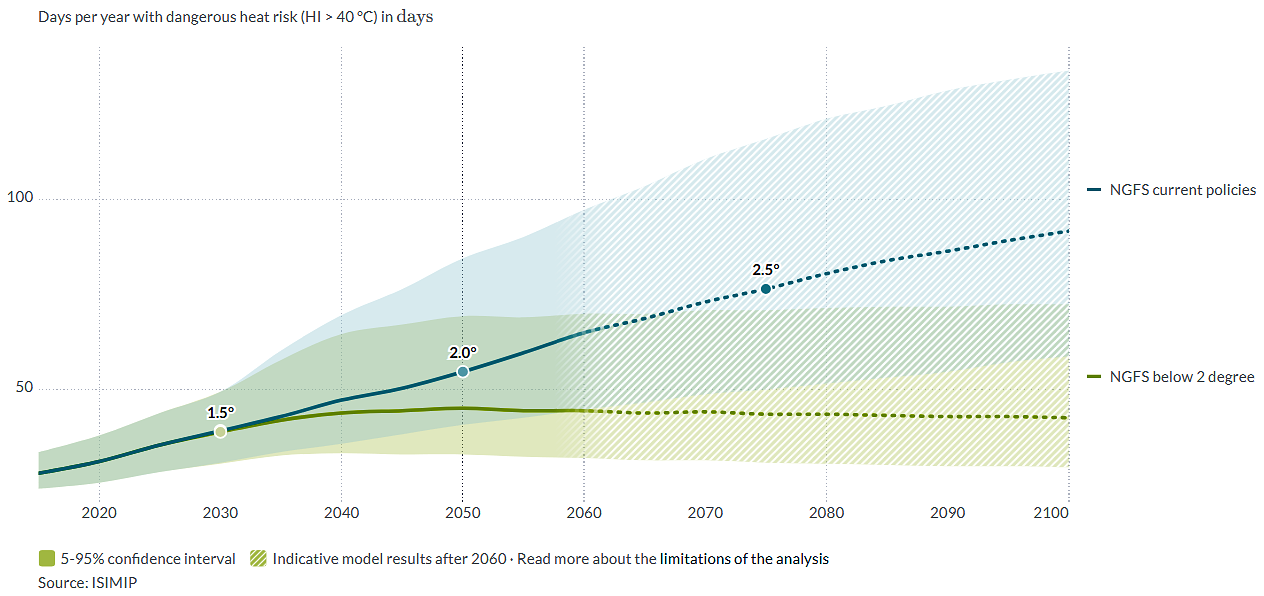
\includegraphics[width=\linewidth]{cie_figure_clean.png}
\caption*{\textbf{Figure 1. Days of dangerous heat per year in Niger, below 2\degC{} (green) and under current
policies (blue).} The curves are identical until about 2030; the gap that opens afterwards is what limiting
warming avoids. Even the low end of the current-policies range in 2100 (59 days) lies above the central
below-2\degC{} value (42 days). Source: Climate Impact Explorer (\CIE).}
\end{figure}
\vspace{-6pt}

\section{Implications for Niger's national interest}
Limiting warming is in Niger's direct interest. Compared with current policies, a below-2\degC{} world would
avoid about 49 days of dangerous heat a year by 2100 and reduce the projected intensification of extreme rainfall
from 43\,\% to 17\,\%; a 1.5\degC{} pathway would keep heat close to today's level. The World Bank estimates that
climate change could reduce Niger's annual GDP by 2.2\,\% in wetter scenarios and by 11.9\,\% in drier ones by
2050 (\WBtwentytwo). These losses can cascade: a hot, dry year cuts harvests and pasture, raises grain prices,
forces households to sell livestock, and can deepen malnutrition and tensions between farmers and herders.
Because drought is projected to spread in every scenario, Niger should defend the 1.5\degC{} goal in the
negotiations while seeking adaptation finance for drought-tolerant crops, water harvesting and early warning.

\section{Uncertainty}
These figures are projections, not forecasts, and model ranges are wide (59 to 134 heat days in 2100 under
current policies). The heat index relies on an estimate of humidity, and the drought indicator counts a single
month of drought, so it saturates. Given Niger's high vulnerability, actual impacts may exceed what these hazard
indicators suggest.

% =====================================================================
%  REFERENCES (page 3, outside the 2-page limit)
% =====================================================================
\clearpage
\section{References}
{\singlespacing
\begin{list}{}{\leftmargin=1.4em \itemindent=-1.4em \itemsep=6pt \parsep=0pt}
\item Climate Analytics (2026). \emph{Climate Impact Explorer}: Niger. Indicators: days per year with dangerous
      heat risk (HI > 40\degC), area under severe drought (SPEI < −1.5) and annual maximum 5-day precipitation;
      NGFS Net Zero 2050, Below 2\degC{} and Current Policies scenarios; ISIMIP data.
      \url{https://climate-impact-explorer.climateanalytics.org} (accessed 9 October 2026).
\item World Bank (2022). \emph{G5 Sahel Region Country Climate and Development Report}. CCDR Series.
      Washington, DC: World Bank. \url{http://hdl.handle.net/10986/37620}
\item World Bank (2024, 28 June). The World Bank supports food security and climate resilience for households
      in Niger [Press release].
      \url{https://www.worldbank.org/en/news/press-release/2024/07/01/the-world-bank-supports-food-security-and-climate-resilience-for-households-in-niger}
\end{list}}

\end{document}
